\begin{tikzpicture}
  \inputdata{power_seq_data}

  \node at (0,-1.5) {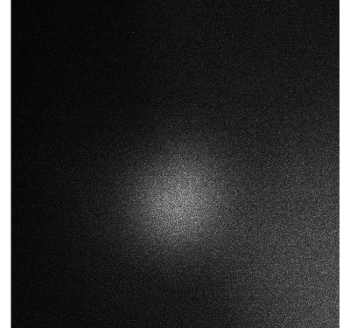
\includegraphics{final-fourier-022.png}};
  \node [white] at (-1, -0.5) {A};
  \draw [thick,->] (6.5,3) -- ++(0,-1.5) node [pos=0,above] {A};

  \node at (3,-1.5) {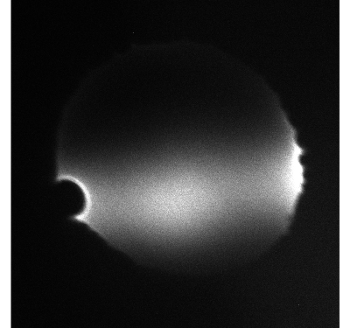
\includegraphics{final-fourier-026.png}};
  \node [white] at (2, -0.5) {B};
  \draw [thick,->] (8,3) -- ++(0,-1.2) node [pos=0,above] {B};

  \node at (6,-1.5) {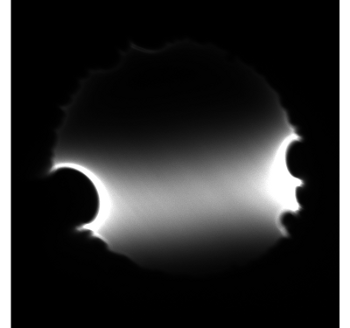
\includegraphics{final-fourier-030.png}};
  \node [white] at (5, -0.5) {C};
  \draw [thick,->] (9,4) -- ++(-80:1.3) node [pos=0,above] {C};

  \node at (9,-1.5) {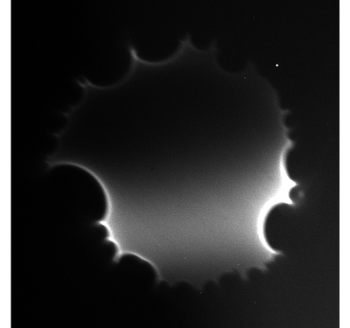
\includegraphics{final-fourier-038.png}};
  \node [white] at (8, -0.5) {D};
  \draw [thick,<-] (11.3,7.5) -- ++(0,-1.5) node [pos=1,below] {D};

  \node at (12,-1.5) {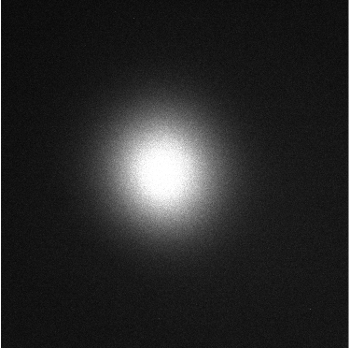
\includegraphics{final-fourier-2photon-036.png}};
  \node [white] at (11, -0.5) {E};
  \draw [thick,->] (11,3) -- ++(0,-1.5) node [pos=0,above] {E};
\end{tikzpicture}
